\documentclass{article} 

\usepackage{hyperref}
\usepackage{graphicx}
\usepackage{subcaption}
\usepackage{caption}

\usepackage{amsmath}
\usepackage{amssymb}

\begin{document}     
\title{Side-Channels in Runtime Systems}
\author{Tegan Brennan\qquad Miroslav Gavrilov}
\maketitle

\section{Side-Channel Analysis}

Any algorithm used in software system must be implemented. It must be written, compiled or interpreted, run on an operating system on certain hardware in some environment. 
By not focusing on the result of the computation, but rather on the side-effects
manifest in this physical implementation, one can gain knowledge of some
implementational details, and thus the structure of the computation itself. Information obtained in this manner is called side-channel information. Side-channels manifest through a large variety of observable properties. For example, the execution time of a program could leak information about which program path was followed or the power trace of a program could correlate with the operations performed. Previously exploited channels include but are not limited to time, power, space, memory, acoustic, and electrogmanetic. 

Side-channel attacks have been increasingly demonstrated as a threat to the confidentiality of private user information. \cite{brumley2005remote, brumley2011remote, hund2013practical, mangard2008power,messerges2000using}. Despite this, programmers remain largely unaware of their threat and there is a dearth of usable tools for their detection let alone preventative. 


\subsection{Outline}
Since runtime systems are complex architectures built for speed, they have the potential to introduce many observable side-channels. Our exploration of side-channel vulnerabilites in runtime systems was guided by the following questions:
\begin{itemize}     
	\item{How does the runtime impact the side-channels found in a program?}
	\item{How do we analyze side-channels?}
	\item{How does language design influence observable side-channels?}
\end{itemize}

The answers to these questions could give an idea of how certain implementation
details decide on how suitable a runtime or language is for tasks that need a level
of discretion in lieu of a potential side-channel as well as some insight into potential future methods for the detection and prevention of side-channels. 


\section{Experiments}

Our analysis was driven through experimentation with various programs containing side-channels of differing strengths. We will briefly describe our experimental setup, highlight some of our most interesting findings, and describe our contribution to the area of side channel detection. The tools we created for this
project are currently in development and open-sourced. 


\subsection{Setup}

All of our experiments have been run on the Java Virtual Machine (Java HotSpot 
64-bit Server), on a 7th generation Intel Core i7 at 3.8GHz with 4 cores and 32GB of RAM.

To showcase side-channels, we select to focus on timing side-channels, as they are common
and easily observable by direct measurement. As we're measuring time on a method-call level, 
we created a driver which, using \texttt{System.nanoTime()}, measures various method lengths,
via calling a single interface method, which many implementations of our examples override. 

We demonstrate our results using several versions of a single program, \texttt{PasswordChecker}
which is a well-known example of timing side-channels. All source code is listed in the appendix.

\texttt{PasswordChecker.checkPassword(input)} is a method with simple semantics: given a public 
\texttt{input}, if a \texttt{secret} value exists, not present in any direct input-output flow, the 
method returns whether \texttt{input} is, character for character, equal to \texttt{secret}.

Different implementations of \texttt{PasswordChecker} have different behaviours. For example,
the na\"ive implementation that would be built for speed, includes early returns as soon as
it is clear that either the lengths of the two strings are different, or that a character
mismatch happened at a certain position. If we try to represent the time needed by the method
to finish, we can write it as $T = t_{len} + n\cdot t_{match} + \epsilon$, where $t_{len}$ is the time needed for
checking the lengths of the two strings, $t_{match}$ is the time needed to match two characters, and $\epsilon$ is the noise in the measurement. We consider that $\epsilon \ll \texttt{min}(t_{len}, t_{match})$, or that the information lost as a result of $\epsilon$ being present is recoverable through taking multiple samples.

We can notice that all the results of our measurements of $T$ can be put into at most $l$ equivalence classes, where $l = \texttt{length}(\texttt{secret})$. By knowing this, we can engineer a side-channel
attack where we can generate the \texttt{secret} by first ascertaining its length and then learning each character in turn. Once the length is known, the first character can be learnt by iterating over all possible values for the character and observing when we access a higher equivalence class (i.e. the program takes longer to execute). The process can be repeated for subsequent characters until the full \texttt{secret} has been leaked.

\texttt{PasswordChecker} can also be implemented in constant time using the XOR operator. This implementation choice removes the side channel resulting from the optimization previously discussed. Figures illustrating both the side channel in the na\"ive implementation as well as its disappearance are provided in the appendix. To accurately analyze timing information, we ran each version of \texttt{PasswordChecker} a million times. Choices for both the secret and the user's guess were drawn at random from a dictionary. To isolate the timing side channel, the length of the two strings are not compared. Instead we ensure that both are of at least length four and the first four characters are compared character-wise. To ensure reliable timing information, we allow for a burn-in period of 100,000 samples before considering the information reliable. Experimentally, this seems to be far more than enough time to allow any compiler optimizations to occur. When analyzing our data, we use a simple outlier detection method based on the average and standard deviation to remove suspect data.   


%By rewriting this, we can decrease the information leak, at the cost of speed. Our main interest is in
%exploring ways in which a runtime system can be better or worse for exploiting side-channels, be it by
%ways of special bytecode, in which side-channel noise is greater by default, special language constraints
%or constructs, that make programmer-created side-channels harder to make, or side-channel specific optimizations or mechanisms.


\subsection{Methods of side-channel detection}

The presence or absence of certain types of side channels can be found by 
statically analyzing the structure of the program in question. For example, the vulnerability in na\"ive \texttt{PasswordChecker} is characterized by the shape of its control flow where obvious length
differences can be observed if we unroll the loop and count how many instructions there are in the resultant
paths. This inspired us to develop a tool to analyze the costs of possible paths through a control flow graph. 

As a first step, we searched for a tool to extract control flow graphs which had several properties we found important: $i$) functional minimality, $ii$) no dependency overhead, and $iii$) modularity and elasticity. Having found no tools that satisfy all three of these, we decided to build our own\footnote{Conflow, \href{https://goo.gl/FnomgF}{https://goo.gl/FnomgF}}, which enabled us to extract control-flow graphs at different levels of abstraction. It is written as a server-client tool, in the hopes of accumulating control-flow data in more than one research field and project; its development will be continued.

We then defined a cost model that acts as a static approximation of our observable value. As we were concerned with timing side-channels, we decided to use the number of bytecode instructions as our cost model and we extracted this information for each basic block in our control flow graph. Given this cost model, each node and back edge of the control flow graph can be annotated with a symbolic expression that provides an over-approximation of all possible cost values that could occur at that node. Boolean variables are introduced for each branch of the program and integer variables for each loop. This allows us to express the possible time spent in a branch, loop, or method symbolically in terms of those variables. 

Possible costs, at this point, can be compared using an off-the-shelf SMT-solver\footnote{$Z3$, for example}, basically solving for any valuation of the variables present that would make the difference in the costs of paths larger than some $\delta$. Using taint analysis, it is possible to determine which branch conditions can be influenced by confidential information. This would allow us to refine our analysis by requiring that the two paths differ only on branch conditions impacted by secret information. 

This static method can inform us of any shape-dictated side-channels occurring in the program, however it is weakened by any form of code transformations, be it the JIT, optimizations or, in scripting languages, obfuscation. Our full implementation of this path cost analysis is still ongoing, but we have made good progress towards a completed tool. 



\subsection{Runtime options and their effect on side-channel strength}
To explore how the runtime options impact runtime we implemented another variant of \texttt{PasswordChecker}. In this version, we introduce two flags initialized to true. All characters are compared. Whenever they don't match the first flag is set to false; whenever they do, the second one is. We analyzed the resulting bytecode in order to ensure that the number of bytecode instructions in both branches was identical. 

Because of this balance, our shape-based anaysis described above would consider the program safe. However, running the same experiment as before resulted in a clear side channel! The figure for this side channel is provided in the appendix. We were not immediately sure of the reason for this, so we decided to disable JIT and re-experiment in the hopes of gaining more insight. In this case, not only did each run take almost two orders of magnitude longer, but the side chanenl dissapeared!

We found this very interesting and hypothesized that the reason behind it might be because the branch taken when two characters are no equal is much more frequently executed than the other. Thus, an optimization introduced by branch prediction may be responsible for this side channel. We were unable to turn off branch prediction but we did run another experiment to help understand this behavior. This time we modified the distribution of guesses for the password so that the first character was guessed correctly approximately 50 percent of the time. When we ran these experiments with JIT-enabled, there was no longer a side channel. We believe that this confirms our hypothesis that the reason for the side channel is branch prediction based on how much more frequent one branch is. Another unexpected consequence is that the user's interaction with the system can impact the presence and strengths of side channels. One distribution of guesses resulted in compiler optimizations that introduced a vulnerability while another did not. We have not yet been able to fully explore this dimension of side-channel analysis but to our knowledge it is an that has not yet been explored in the literature and which we believe could lead to new exploits. 





\subsection{Differences in side-channels due to language design}

To explore how different language syntax behaves with side-channels, we compared the implementation of \texttt{PasswordChecker} in Java and in Scala. Both languages share the JVM, although Scala is usually written in a mostly functional manner. The result of this paradigm shift is that most of the instructions found in Scala bytecode are method calls, presented in the bytecode as artificial anonymous classes, and subject to a large array of Scala analyses and optimizations at compile-time. This causes the side-channel to not appear, if written in the way most Scala programmers would typically align themselves with.

% scala diagram (just the normal one, the par is kinda contrived)

From this, we can see that the choice of valid language syntax and semantics based on formalism and consistency can help improve side-channel prevention, even though it isn't necessarily looking to solve that problem. The main reason behind why the side-channel isn't present in the Scala code is that all traversals through the sequence of characters are designed to be exactly $n * O(1)$, where $n$ is the length of the array, instead of being $O(n)$, as is the case with languages that allow early-returns, as is Java. Furthermore, if an attempt be made to write Java-like loops in Scala, a weak space side-channel could form as well, as the early break mechanisms are implemented via lazy structures, thus holding the rest of the calculation in memory while evaluating the start of the sequence. It follows that good performance strongly follows good practice in this case.

\section{Discussion}

In our exploration of timing side-channels, a repeated observation was that vulnerabilities were introduced from atemptes at optimization, whether by the programmer or the compiler. 
This phenomenon builds a kind of philosophical construct similar to the Heisenberg
uncertainty principle wherein the limitations of our physical reality are stopping
us from being both optimized (take less time in most cases) and, for example, 
completely computationally private (as observed in \cite{archlab-timing-14}). The
case in which the least side-channel activity is present is the case in which the 
lengths of all the possible routes of execution of the main-channel are of similar
size, and thus observation becomes noisy in the presence of other physical factors.
This, unsurprisingly, is the case in which there is no optimization made and all the
lengths are similar to the longest one.


%to be cleaned up

%mainly discuss optimization versus safety 
%optimization on many levels, programmer versus compiler

\pagebreak
\bibliographystyle{unsrt}
\bibliography{biblio}

\pagebreak
\section{Appendix}

\subsection{Code}

\subsubsection{PasswordChecker}

\begin{figure}[h]
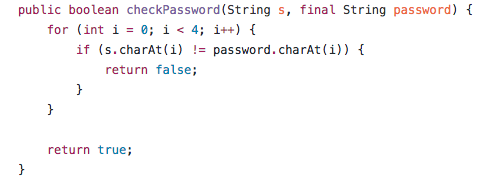
\includegraphics[width=.7\linewidth]{code/insecure.png}
\caption{Code for the na\"ive version of \texttt{PasswordChecker}.}

\end{figure}

\begin{figure}[h]
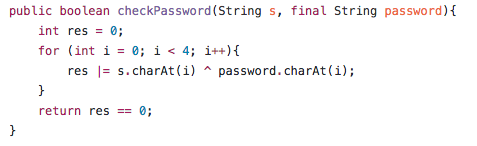
\includegraphics[width=.7\linewidth]{code/constant.png}
\caption{Code for the constant-time version of \texttt{PasswordChecker}.}

\end{figure}

\begin{figure}[h]
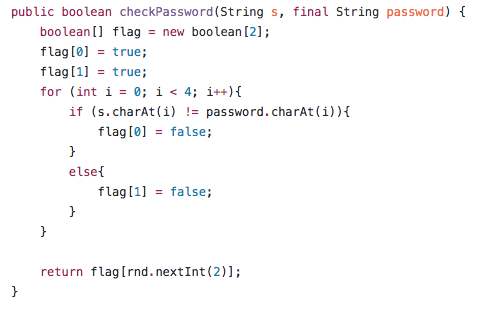
\includegraphics[width=.7\linewidth]{code/branches.png}
\caption{Code for the balanced-branches version of \texttt{PasswordChecker}.}

\end{figure}

\pagebreak


\subsubsection{Inlining Experiments}
\begin{figure}[h]
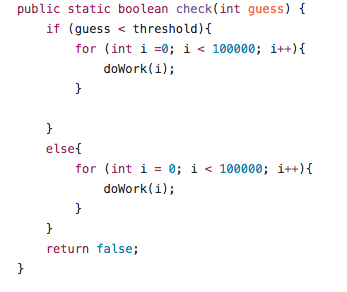
\includegraphics[width=.7\linewidth]{code/inline.png}
\caption{Code used for the inlining experiments.}
\end{figure}

\pagebreak


\subsection{Figures}

\begin{figure}[h]
\centering
\begin{subfigure}{.5\textwidth}
  \centering
  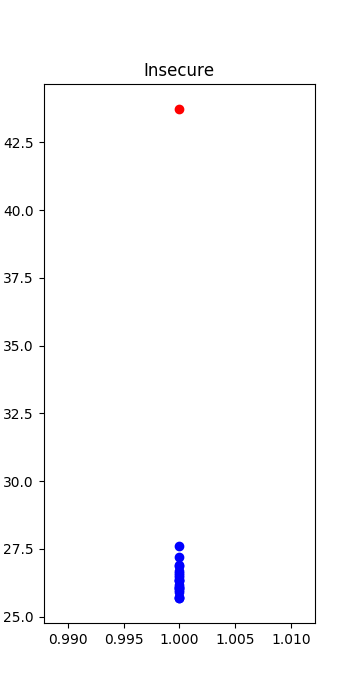
\includegraphics[width=.7\linewidth]{figures/insecure0.png}
  \caption{Na\"ive implementation}
  \label{fig:sub1}
\end{subfigure}%
\begin{subfigure}{.5\textwidth}
  \centering
  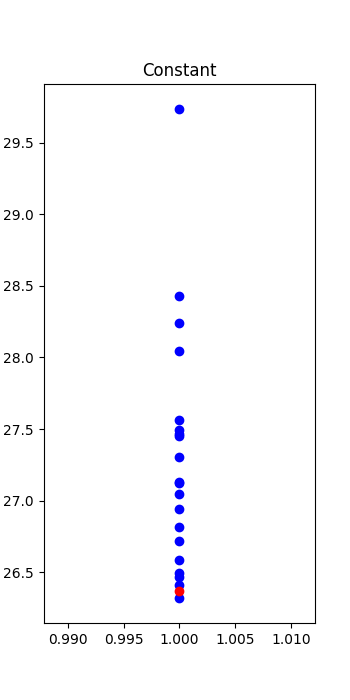
\includegraphics[width=.7\linewidth]{figures/constant0.png}
  \caption{Constant Time implementation}
  \label{fig:sub2}
\end{subfigure}
\caption{Comparison of side-channel vulnerability between the na\"ive and constant time implementations of \texttt{PaswordChecker}. In each figure, the dots are each the time taken for a sample parameterized by the first character of the user guess. The red data point is the resulting time when the first character of the guess matches that of the secret.}
\label{fig:test}
\end{figure}

\begin{figure}
\centering
\begin{subfigure}{.5\textwidth}
  \centering
  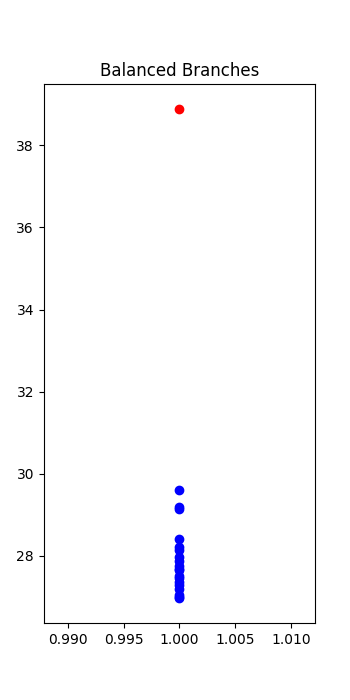
\includegraphics[width=.7\linewidth]{figures/branches0.png}
  \caption{With JIT}
  \label{fig:sub1}
\end{subfigure}%
\begin{subfigure}{.5\textwidth}
  \centering
  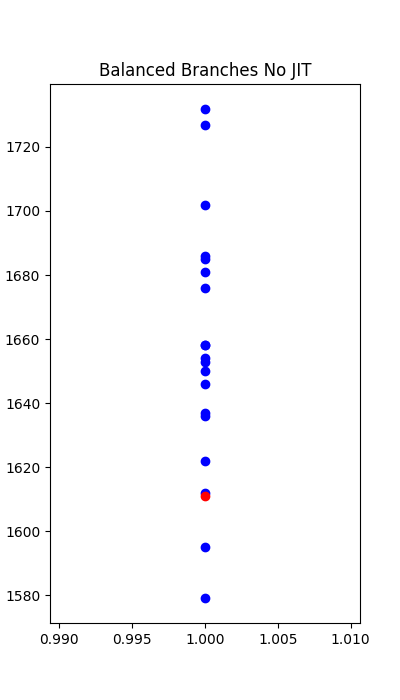
\includegraphics[width=.7\linewidth]{figures/nJITbranch1.png}
  \caption{Without JIT}
  \label{fig:sub2}
\end{subfigure}
\caption{Comparison of side-channel vulnerability for the balanced path \texttt{PassswordChecker} with and without JIT enabled. In each figure, the dots are each the time taken for a sample parameterized by the first character of the user guess. The red data point is the resulting time when the first character of the guess matches that of the secret.}
\label{fig:test}
\end{figure}

\begin{figure}
\centering
\begin{subfigure}{.5\textwidth}
  \centering
  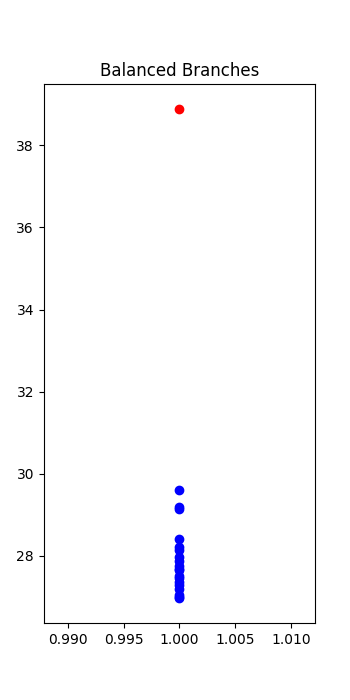
\includegraphics[width=.7\linewidth]{figures/branches0.png}
  \caption{Original input distribution}
  \label{fig:sub1}
\end{subfigure}%
\begin{subfigure}{.5\textwidth}
  \centering
  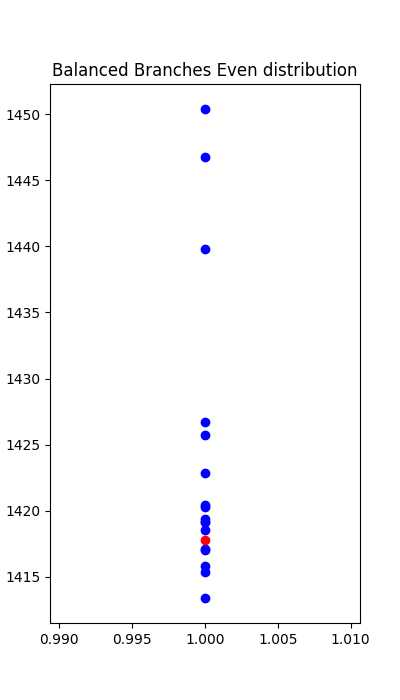
\includegraphics[width=.7\linewidth]{figures/distribution_branches2.png}
  \caption{Modified input distribution}
  \label{fig:sub2}
\end{subfigure}
\caption{Comparison of side-channel vulnerability for the balanced path \texttt{PassswordChecker} with a modified input distribution versus the original. In each figure, the dots are each the time taken for a sample parameterized by the first character of the user guess. The red data point is the resulting time when the first character of the guess matches that of the secret.}
\label{fig:test}
\end{figure}

\begin{figure}
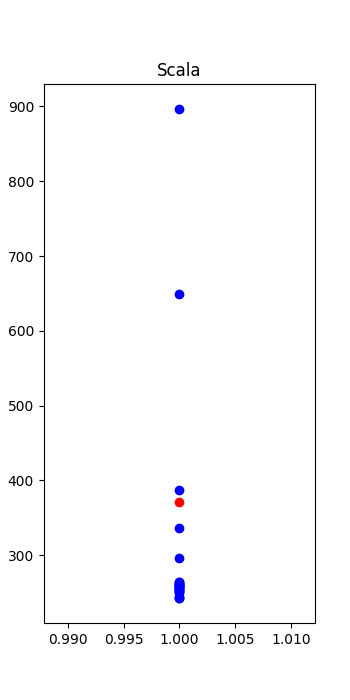
\includegraphics[width=.7\linewidth]{figures/scala.png}
\caption{Results of the side-channel vulnerability for our scala implementation.}
\end{figure}




\end{document}
